Background

How do we evaluate a model like this
There are no established protocols (few references?)
One way would be to put personal monitoring equipment on all the people in the model, and evaluate the data against the model predictions
But this would be too expensive
In addition, the micro environmental factors introduce further uncertainty to the model
If we simplify the problem, we know that CMAQ produces reasonable predictions of outdoor air quality
GRAPHS
To see how well cmaq performs at a monitoring site, we take a full year of data from the site, then calculate annual average weekday/sat/sun hourly values, and compare to the model, at the location of the site.
How well does CMAQ perform away from monitoring sites though? 
Without creating monitoring sites in every 20 metre grid square around London, we can't
Monitoring sites can predict the temporal variation in air quality reasonable well, but the spatial aspect??
Can we use mobile monitoring equipment to attempt this evaluation? 
We decided to test this hypothesis using one of the cyclist journeys from the LHEM. But we can't continuously sample a route all year every hour to get a annual average figure like is used in cmaq and the monitoring site data. So we'll need to make this collection reasonable. This is covered in methods below.
Once we know how many samples we'll need to take, and how to make this into an annual average, we'll need to actually do the sampling. We will then explore the relationship between the modelled cmaq concentrations, and the data collected, spatially (is the pattern right?) and in terms of overall concentrations.

Methods

Collecting data representative of an annual average -- we can't sample all year. we theorised that we could sample X times within a timeframe, to be representative of that timeframe, and then using scaling factors from the monitoring site, to expand that data to be a year. The cmaq data is weekday/sat/sunday hourly annual average. So to simplify we are going to evaluate weekdays, from 9am to 10am. Given this, we decided we'd do the sampling between August and September 2017, 9am to10am. So how many samples are we going to need to be representative of 9am to 10am, between this period, on weekday mornings? We took minute by minute NO2 data from putney, did sums, see table, decided on 27. We used NO2 because minute level PM2.5 data was not available.

Where will we collect the data -- Wanted to make the data collection unobtrusive to the life of the person who would do it. 27 times within 45 days. Needed to make it regular. Decided to sample a cycle journey that can be managed regularly and sampled enough times. Choose researchers commute from Kennington Park to the King's College Building. Here's a pic of the route.

Mobile monitoring equipment -- we do not have any mobile NO2 instruments that can collect data on a minute basis. So we decided to use black carbon, and then convert this to NO2, given we know that they strongly correlate in London. We used this instrument to do the collection. To calculate the conversion from black carbon to NO2, we took data from Putney monitoring site in London, as it has simultaneous bc and NO2 data. Here it is. This is the conversion we calculated. We applied it to the black carbon data.

Spatial aggregation -- We wanted to be able to calculate

Results







%%%%%%%%%%%%%%%%%%%%%%%%%%%%%%%%%%%%%%%%%%%%%%%%%%%%%%%%%%%%%%%%%%%%%%%%%%%%%%%%%%%
\section{Background}
\label{sec:4background}
%%%%%%%%%%%%%%%%%%%%%%%%%%%%%%%%%%%%%%%%%%%%%%%%%%%%%%%%%%%%%%%%%%%%%%%%%%%%%%%%%%%

%The focus of this PhD research so far has been on developing a dynamic exposure model to better understand exposure to urban air pollution in the population of London. Having reconstructed the %time-activity of the population, their exposure was modelled, and then refined, with further investigation of the London Underground micro-environment. This next chapter will consider how to %evaluate the results that are calculated using an exposure model of this type, and then attempt to do this by taking some measurements using personal monitoring equipment.
%
%Evaluating the performance of the LHEM model predictions has already occurred to some degree, within each of the constituent parts of the model. For example the CMAQ-UK air quality input is %evaluated against air quality monitoring stations, and the indoor air quality and in-vehicle air quality aspects of the model have been qualitatively compared to literature on concentrations in %these environments (\cite{Smith2016}) n.b. the in-vehicle module of the model has been recently updated, and now uses vehicle specific scaling ratios from a Lancet review in 2017 %(\cite{Cepeda2017}), instead of the mass-balance model. This decision was taken as whilst the theoretical approach of a mass-balance model was sound, the output tended to result in concentrations %almost identical to the outdoor concentrations taken from the CMAQ-UK input, whereas empirical research suggested that this should not be the case.%
%
%So whilst some qualitative evaluation of specific concentrations and micro-environments has occurred, this chapter aims to consider how to evaluate the exposure modelling of journeys and trips, the %variability within them, and possible reasons for disagreement. Primarily because we saw earlier in this research (Figure \ref{fig:lhem_address_whether_leave_house}) that leaving the home and %encountering transport microenvironments were a key factor in the difference between static and dynamic exposure estimates. Within the exposure modelling of trips, there are a number of %micro-environment's modelled; indoors, walking, cycling, in-car, in-bus, in-tube and in-train. To attempt to evaluate the LHEM predictions of all these environments would be a large research %project, and therefore the decision was taken to concentrate on outdoor exposure, on weekdays i.e. cycling and walking on Monday-Friday. This should make the evaluation more manageable, as the LHEM %model takes these predictions directly from the CMAQ-UK air quality model, without further micro-environmental modelling being applied e.g. indoor/outdoor/transport ratios. By undertaking %evaluation of this small aspect of a dynamic model it is hoped to better understand how a full evaluation of a dynamic model might be undertaken.

%%%%%%%%%%%%%%%%%%%%%%%%%%%%%%%%%%%%%%%%%%%%%%%%%%%%%%%%%%%%%%%%%%%%%%%%%%%%%%%%%%%
%\section{Methods}
%\label{sec:4methods}
%%%%%%%%%%%%%%%%%%%%%%%%%%%%%%%%%%%%%%%%%%%%%%%%%%%%%%%%%%%%%%%%%%%%%%%%%%%%%%%%%%%

%% want to consider how to start evaluation of hybrid models
%% Our lhem model uses annual, weekday/sat/sun, hourly cmaq data as input
%% we're going to do cycling journeys as it removes the potential errors of the mass-balance equation might introduce. We're just using 'raw' cmaq data.
%% want to estimate repeat journey numbers to be representative. how many?
%% need minute data to calculate this as that's what personal monitor records
%% it's basically a statistical power calculation
%% we need a reliable verified dataset to calculate this with
%% use putney high street no2 ( ENPutneyAethalometer.dbo )
%% Find it's <10> repeat samples of 9am data throughout the year to get an annual average for that day, so that's the number of repeat trips we'll do
%% %% We/studies can't do randomly as above though, it's impractical for reasons X, y, z
%% So we are going to do all <10> within August instead. We will then calculate the monthly variation using the same monitoring site data, and apply that to our data, to %% turn it into annual average 'journey' and exposure. So we need to go do the sampling now...
%% %% But we don't have a portable reliable NO2 sensor. We do have black carbon though. Black carbon is well correlated with NO2 (graphs, conversion factor etc).
%% So we measure black carbon using a microaeth ten times. Do the maths to make it annual.
%% %% Now we do the same journey using the LHEM model.
%% Start doing some comparisons.


%%%%%%%%%%%%%%%%%%%%%%%%%%%%%%
%\subsection{Estimating repeat journey numbers}
%\label{evaluation_journey_numbers}
%%%%%%%%%%%%%%%%%%%%%%%%%%%%%%

%Having refined the aspects of the LHEM that we intend to evaluate, to outdoor cycling journeys on a weekday, we needed to consider how many repeat samples of the same journey would give a %representative or 'typical' exposure for that journey. Just taking measurements on a single journey at a convenient time and then comparing those measurements to our model predictions would be %difficult to compare fairly as the CMAQ-UK model outputs concentrations as an annual, daily (weekday/Saturday/Sunday), hourly average; and we would not be able to say with any certainty that the %personal monitoring we have undertaken was representative of the typical annual, daily, hourly exposure CMAQ-UK was outputting. Therefore, we decided to replicate the hour of the day and whether it %was a weekday or weekend that the journey occurred on, when doing the personal sampling. So now we are at least, for instance, comparing 11am on a Monday with 11am on a Monday. However we were %still left with the question of whether the 11am Monday we are sampling on, is representative of typical 11am on Monday's concentrations. To attempt to answer this, we used a power and sample size %equation i.e. how many exposures/journeys are needed to be representative of the annual weekday average exposure/journey on that route at that time of day and day of the week. Linked to this, once %we have determined how many samples are needed to represent an annual weekday hourly average, we have a further practical issue, that within the scope of this research we cannot sample all year. We %therefore set the sampling period as 1 August 2017 to 30 November 2017, weekdays, between 9am and 10am, to be convenient for data collection. These samples, once we have calculated how many are %needed, will then be scaled to be representative of the entire year based on a yearly profile from monitoring site data. The method and rationale behind this process is clearly open to debate and %further investigation, but as there are no published methods suitable for evaluating an exposure model of this type we decided that this approach was at least reasonable. The limitations and %presumptions are discussed more later.

%To attempt to answer the question of how many samples are needed within the sampling period to be representative of a typical weekday 9am to 10am concentration within this period, we needed a continuous, minute resolution, sample of the pollutant we are interested in evaluating. This resolution of data is not typically captured by the London Air Quality Network, however at the site 'Wandsworth - Putney High Street' there is one minute NO$_{2}$ data for the year 2015 available, so we decided to base our calculations on this (recognising that 2017 data would be preferable, but not being available). The following steps were then completed:

%\begin{enumerate}
%   \item Download NO$_{2}$ minute-resolution data from site WA7 for 2015
%   \item Discard data outside of sampling period (1 August 2015 to 30 September 2015)
%   \item Discard weekends
%   \item Discard data outside of 9am-10am
%   \item Calculate summary statistics.
%\end{enumerate}

%The results of the process outlined above are shown in Table \ref{tab:wa7_summary_stats} below.
%
%\begin{table}[H]
%\centering
%    \begin{tabular}{ | l | l |}
%    \hline 
%     \bfseries{Statistic}   & \bfseries{NO$_{2}$ $\mu \text{g m}^{-3}$}    \\ \hline
%     Minutes                & 2400                                         \\ \hline
%     Mean                   & 90.92                                        \\ \hline
%     Median                 & 77.70                                        \\ \hline
%     Max                    & 1074.4                                       \\ \hline
%     Min                    & 11.67                                        \\ \hline
%     Standard deviation     & 64.23                                        \\ \hline
%    \end{tabular}
%\caption{Site WA7 summary statistics for weekday, 9am-10am during}
%\label{tab:wa7_summary_stats}
%\end{table}

%Now that we have summary statistics for the period of time we are interested in, we can calculate how many samples are required within this period to adequately represent the period using Equation %\ref{eq:sample_size_equation_pt1} (\cite{PennStateEberlyCollegeofScience2017}). By taking this reliable and continuous dataset, in a known location, we extrapolate it's findings to be %representative of a non-fixed site data collection method.

%\begin{equation}
%  \chi = \textit{Z}^2 \times \frac{\sigma^2}{moe^2} 
%  \label{eq:sample_size_equation_pt1}
%\end{equation}
%
%Where $\chi$ is the calculated sample size, \textit{Z} is the z-score of the desired confidence level, $\sigma$ is the standard deviation of the population (concentrations), and \textit{moe} is the %allowed margin of error (in $\mu \text{g m}^{-3}$). By writing a loop in the R programming language (\cite{RFoundationforStatisticalComputing2014}), and testing a variety of input variables to this %equation, we were able to see how many samples would be required in different scenarios of confidence levels and allowable margins of error. The results are shown in Table %\ref{tab:no2_samples_needed}:

%\begin{table}[H]
%\centering
%\begin{tabular}{|l|l|l|}
%\hline
%Confidence Interval     &            Allowed margin of error                            &        Sample required       \\ \hline
%\multirow{6}{*}{99\%}   &            10\% ($\pm$ 9   $\mu \text{g m}^{-3}$ )    &        1325                  \\ \cline{2-3} 
%                        &            15\% ($\pm$ 14  $\mu \text{g m}^{-3}$ )    &        589                   \\ \cline{2-3} 
%                        &            20\% ($\pm$ 18  $\mu \text{g m}^{-3}$ )    &        331                   \\ \cline{2-3}
%                        &            25\% ($\pm$ 23  $\mu \text{g m}^{-3}$ )    &        212                   \\ \cline{2-3}
%                        &            30\% ($\pm$ 27  $\mu \text{g m}^{-3}$ )    &        147                   \\ \cline{2-3}
%                        &            35\% ($\pm$ 32  $\mu \text{g m}^{-3}$ )    &        108                   \\ \hline
%\multirow{6}{*}{95\%}   &            10\% ($\pm$ 9   $\mu \text{g m}^{-3}$ )    &        767                   \\ \cline{2-3} 
%                        &            15\% ($\pm$ 14  $\mu \text{g m}^{-3}$ )    &        341                   \\ \cline{2-3} 
%                        &            20\% ($\pm$ 18  $\mu \text{g m}^{-3}$ )    &        192                   \\ \cline{2-3} 
%                        &            25\% ($\pm$ 23  $\mu \text{g m}^{-3}$ )    &        123                   \\ \cline{2-3} 
%                        &            30\% ($\pm$ 27  $\mu \text{g m}^{-3}$ )    &        85                    \\ \cline{2-3} 
%                        &            35\% ($\pm$ 32  $\mu \text{g m}^{-3}$ )    &        63                    \\ \hline
%\multirow{6}{*}{90\%}   &            10\% ($\pm$ 9   $\mu \text{g m}^{-3}$ )    &        540                   \\ \cline{2-3} 
%                        &            15\% ($\pm$ 14  $\mu \text{g m}^{-3}$ )    &        240                   \\ \cline{2-3} 
%                        &            20\% ($\pm$ 18  $\mu \text{g m}^{-3}$ )    &        135                   \\ \cline{2-3} 
%                        &            25\% ($\pm$ 23  $\mu \text{g m}^{-3}$ )    &        86                    \\ \cline{2-3} 
%                        &            30\% ($\pm$ 27  $\mu \text{g m}^{-3}$ )    &        60                    \\ \cline{2-3} 
%                        &            35\% ($\pm$ 32  $\mu \text{g m}^{-3}$ )    &        44                    \\ \hline
%\multirow{6}{*}{85\%}   &            10\% ($\pm$ 9   $\mu \text{g m}^{-3}$ )    &        414                   \\ \cline{2-3} 
%                        &            15\% ($\pm$ 14  $\mu \text{g m}^{-3}$ )    &        184                   \\ \cline{2-3} 
%                        &            20 \% ($\pm$ 18 $\mu \text{g m}^{-3}$ )    &        103                   \\ \cline{2-3} 
%                        &            25\% ($\pm$ 23  $\mu \text{g m}^{-3}$ )    &        66                    \\ \cline{2-3} 
%                        &            30\% ($\pm$ 27  $\mu \text{g m}^{-3}$ )    &        46                    \\ \cline{2-3} 
%                        &            35\% ($\pm$ 32  $\mu \text{g m}^{-3}$ )    &        34                    \\ \hline
%\multirow{6}{*}{80\%}   &            10\% ($\pm$ 9   $\mu \text{g m}^{-3}$ )    &        327                   \\ \cline{2-3} 
%                        &            15\% ($\pm$ 14  $\mu \text{g m}^{-3}$ )    &        145                   \\ \cline{2-3} 
%                        &            20\% ($\pm$ 18  $\mu \text{g m}^{-3}$ )    &        82                    \\ \cline{2-3} 
%                        &            25\% ($\pm$ 23  $\mu \text{g m}^{-3}$ )    &        52                    \\ \cline{2-3} 
%                        &            30\% ($\pm$ 27  $\mu \text{g m}^{-3}$ )    &        36                    \\ \cline{2-3} 
%                        &            35\% ($\pm$ 32   $\mu \text{g m}^{-3}$ )   &        27                    \\ \hline
%\end{tabular}
%\caption{Samples needed}
%\label{tab:no2_samples_needed}
%\end{table}

%For comparison, we then completed this same sample size testing, but for all 9am to 10am  periods on weekdays throughout the whole year, to see whether the results we found for the August to %September period are similar throughout the year. The results of this are shown in Table \ref{tab:no2_samples_needed_whole_year}:

%\begin{table}[H]
%\centering
%\begin{tabular}{|l|l|l|}
%\hline
%Confidence Interval     &      Margin of error                                  &        Sample required       \\ \hline
%\multirow{6}{*}{99\%}   &            10\% ($\pm$    $\mu \text{g m}^{-3}$ )    &                          \\ \cline{2-3} 
%                        &            15\% ($\pm$   $\mu \text{g m}^{-3}$ )    &                           \\ \cline{2-3} 
%                        &            20\% ($\pm$   $\mu \text{g m}^{-3}$ )    &                           \\ \cline{2-3}
%                        &            25\% ($\pm$   $\mu \text{g m}^{-3}$ )    &                           \\ \cline{2-3}
%                        &            30\% ($\pm$   $\mu \text{g m}^{-3}$ )    &                           \\ \cline{2-3}
%                        &            35\% ($\pm$   $\mu \text{g m}^{-3}$ )    &                           \\ \hline
%\multirow{6}{*}{95\%}   &            10\% ($\pm$    $\mu \text{g m}^{-3}$ )    &                           \\ \cline{2-3} 
%                        &            15\% ($\pm$   $\mu \text{g m}^{-3}$ )    &                           \\ \cline{2-3} 
%                        &            20\% ($\pm$   $\mu \text{g m}^{-3}$ )    &                           \\ \cline{2-3} 
%                        &            25\% ($\pm$   $\mu \text{g m}^{-3}$ )    &                           \\ \cline{2-3} 
%                        &            30\% ($\pm$   $\mu \text{g m}^{-3}$ )    &                            \\ \cline{2-3} 
%                        &            35\% ($\pm$   $\mu \text{g m}^{-3}$ )    &                            \\ \hline
%\multirow{6}{*}{90\%}   &            10\% ($\pm$    $\mu \text{g m}^{-3}$ )    &                           \\ \cline{2-3} 
%                        &            15\% ($\pm$   $\mu \text{g m}^{-3}$ )    &                           \\ \cline{2-3} 
%                        &            20\% ($\pm$   $\mu \text{g m}^{-3}$ )    &                           \\ \cline{2-3} 
%                        &            25\% ($\pm$   $\mu \text{g m}^{-3}$ )    &                            \\ \cline{2-3} 
%                        &            30\% ($\pm$   $\mu \text{g m}^{-3}$ )    &                            \\ \cline{2-3} 
%                        &            35\% ($\pm$   $\mu \text{g m}^{-3}$ )    &                            \\ \hline
%\multirow{6}{*}{85\%}   &            10\% ($\pm$    $\mu \text{g m}^{-3}$ )    &                           \\ \cline{2-3} 
%                        &            15\% ($\pm$   $\mu \text{g m}^{-3}$ )    &                           \\ \cline{2-3} 
%                        &            20 \% ($\pm$  $\mu \text{g m}^{-3}$ )    &                           \\ \cline{2-3} 
%                        &            25\% ($\pm$   $\mu \text{g m}^{-3}$ )    &                            \\ \cline{2-3} 
%                        &            30\% ($\pm$   $\mu \text{g m}^{-3}$ )    &                            \\ \cline{2-3} 
%                        &            35\% ($\pm$   $\mu \text{g m}^{-3}$ )    &                            \\ \hline
%\multirow{6}{*}{80\%}   &            10\% ($\pm$    $\mu \text{g m}^{-3}$ )    &                           \\ \cline{2-3} 
%                        &            15\% ($\pm$   $\mu \text{g m}^{-3}$ )    &                           \\ \cline{2-3} 
%                        &            20\% ($\pm$   $\mu \text{g m}^{-3}$ )    &                            \\ \cline{2-3} 
%                        &            25\% ($\pm$   $\mu \text{g m}^{-3}$ )    &                            \\ \cline{2-3} 
%                        &            30\% ($\pm$   $\mu \text{g m}^{-3}$ )    &                            \\ \cline{2-3} 
%                        &            3\% ($\pm$    $\mu \text{g m}^{-3}$ )    &                            \\ \hline 
%\end{tabular}
%\caption{Samples needed}
%\label{tab:no2_samples_needed_whole_year}
%\end{table}

%NNEED TO TALK TO BEN ABOUT THE
%As the journey that we are going to be repeat sampling must be done between 9am and 10am on weekdays (for reasons explained above), within the defined period of 1 August 2017 to 30 September 2017, %the maximum number of samples that could reasonably be taken by one researcher was one a day, giving a maximum of 44 samples in total over the period. Given that taking a sample every day would %likely not be possible due to availability of the equipment, and other commitments meaning that the researcher was not available every day, we decided to select a margin of error and confidence %interval that made conducting the research a reasonable proposition, namely an 80\% confidence interval and a margin of error of 35\%, giving a required sample number of 27. Clearly in most %statistical situations this would be an undesirable level of precision, but there are few precedents for evaluating this type of exposure model, and it may be that this is the sort of confidence %that has to be accepted in these situations. This is explored more in the Section \label{sec:4Discussion}.
%
%%%%%%%%%%%%%%%%%%%%%%%%%%%%%%
%\subsection{Correlations between \texorpdfstring{NO$_{2}$}{} and black carbon}
%\label{no2_pm25_correlations}
%%%%%%%%%%%%%%%%%%%%%%%%%%%%%%

%To complete the NO$_{2}$ personal monitoring of the cycling journeys a lightweight, accurate, portable NO$_{2}$ sensor with high time-resolution was required. However there are no such devices %currently available (BEN? GOT A REF?). Passive NO$_{2}$ samplers are commonly used for research and occupational health purposes, however the highest time resolution available from these devices is %one hour, which will not allow detailed examination of the spatial and temporal differences between the LHEM prediction and the personal monitoring evaluation data being collected. It was suggested %by a colleague that as black carbon and NO$_{2}$ tend to be strongly correlated, that a portable black carbon monitor could be used as a proxy, then the results converted to NO$_{2}$. A short %literature search was undertaken and the following references, and conversation factors, were found ( TABLE X)

%\cite{Vanderstraeten2011}
%\cite{Beckerman2008}
%
%The conversion factors were X, Y, Z so we took the mean and used a conversion factor of X.

%%%%%%%%%%%%%%%%%%%%%%%%%%%%%%
%\subsection{Measuring black carbon using an Aethlabs MA300}
%\label{evaluation_microaeth}
%%%%%%%%%%%%%%%%%%%%%%%%%%%%%%

%A full description of the Aethlabs MA300 is available via their website \url{https://aethlabs.com/microaeth/ma300/overview}. In summary, it is a small real-time optical based black carbon monitor, %with automatic filter advancement, and internal GPS. For the personal monitoring required for this research it was set to a one minute sampling rate, and placed in the backpack of the cyclist with %the inlet tube poking out the top of the cyclists bag. It was turned on at the start of the journey, and turned off at the end. Data was periodically downloaded from the device using the provided %software, and imported to R for analysis.

%%%%%%%%%%%%%%%%%%%%%%%%%%%%%%
%\subsection{Journey choice for evaluation}
%\label{journey_evaluation_choice}
%%%%%%%%%%%%%%%%%%%%%%%%%%%%%%

%As the journey we sampled would need to be sampled at least 27 out of the 44 days available in the sampling period, we decided to fit this around the researchers schedule, and selected a cycling %journey that they would be doing anyway i.e. a portion of their home to work commute. This is shown in Figure \ref{fig:cycling_busy_route}).

%\begin{figure}[H]
%\centering
%  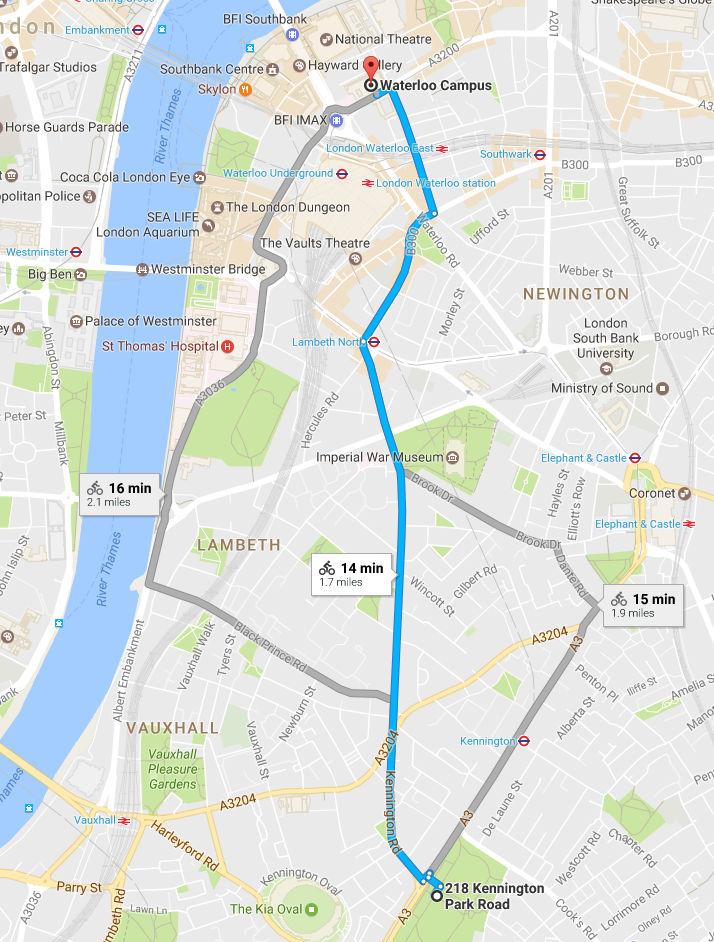
\includegraphics[scale=0.8]{cycling_busy_route}
%  \caption{A cycling journey from Kennington Park to the Franklin-Wilkins Building of King's College London}
%  \label{fig:cycling_busy_route}
%\end{figure}

%%%%%%%%%%%%%%%%%%%%%%%%%%%%%%
%\subsection{Microaeth MA300 data export}
%\label{evaluation_location_diary}
%%%%%%%%%%%%%%%%%%%%%%%%%%%%%%

%The sampling of journeys was completed during the period, the data exported from the MA300 to individual CSV files, and then the files combined into one data frame object in R for analysis. Many of %the variables that the MA300 outputs were not required for analysis and were discarded, leaving the variables of latitude, longitude, black carbon, sample number, date and time. A sample of the %data is shown in TABLE XX.

%TABLE HERE.

%%%%%%%%%%%%%%%%%%%%%%%%%%%%%%%%%%%%%%%%%%%%%%%%%%%%%%%%%%%%%%%%%%%%%%%%%%%%%%%%%%%
%\section{Results}
%\label{sec:4results}
%%%%%%%%%%%%%%%%%%%%%%%%%%%%%%%%%%%%%%%%%%%%%%%%%%%%%%%%%%%%%%%%%%%%%%%%%%%%%%%%%%%

%First section will be comparing minutes past a monitor to get annual / hourly averages. Establishes number of journeys needed. Do a few different monitors / times / seasons maybe.
%Results of the personal monitoring of X journeys. Explore.
%Calculate average exposure for those journeys + compare to the LHEM output for the same journey. Explore.

%%%%%%%%%%%%%%%%%%%%%%%%%%%%%%%%%%%%%%%%%%%%%%%%%%%%%%%%%%%%%%%%%%%%%%%%%%%%%%%%%%%
%\section{Discussion}
%\label{sec:4Discussion}
%%%%%%%%%%%%%%%%%%%%%%%%%%%%%%%%%%%%%%%%%%%%%%%%%%%%%%%%%%%%%%%%%%%%%%%%%%%%%%%%%%%

%include suggestions for refining LHEM
%needs to discuss how personal monitoring is the average of a minute of space, but modelling is a snapshot minute in space. 
% For instance gaining a 95\% confidence level with a 10\% margin of error would require 767 samples in 44 days, ~17 samples a day, which unless the team has an army
 
%BUS / TUBE / WHY WE NEED INFRASTRUCTURE TO DO THE REPEATS.

%%%%%%%%%%%%%%%%%%%%%%%%%%%%%%%%%%%%%%%%%%%%%%%%%%%%%%%%%%%%%%%%%%%%%%%%%%%%%%%%%%%
%\section{Conclusions}
%\label{sec:4conclusions}
%%%%%%%%%%%%%%%%%%%%%%%%%%%%%%%%%%%%%%%%%%%%%%%%%%%%%%%%%%%%%%%%%%%%%%%%%%%%%%%%%%%